% =============================================================================
% Section 5.3: Test Schedule
% =============================================================================

\section{Test Schedule}
\label{sec:test-schedule}

The testing activities were phased across the development lifecycle, aligned with the six-week sprint structure used for the project. Table~\ref{tab:test-schedule} presents the schedule in a Gantt-style format showing the start week, duration, and current status of each testing phase.

\begin{table}[H]
  \centering
  \caption{Testing Schedule Across Development Phases}\label{tab:test-schedule}
  \small
  \begin{tabular}{lccc}
    \toprule
    \textbf{Phase}                        & \textbf{Start Week} & \textbf{Duration} & \textbf{Status} \\
    \midrule
    Unit test framework setup             & 1                   & 1 week            & Completed    \\
    Domain entity unit tests (Auth)       & 1                   & 1 week            & Completed    \\
    Domain entity unit tests (Courses)    & 1                   & 1 week            & Completed    \\
    Domain entity unit tests (Media)      & 1                   & 1 week            & Completed    \\
    Domain entity unit tests (Assessment) & 2                   & 1 week            & Completed    \\
    Domain entity unit tests (Payment)    & 2                   & 1 week            & Completed    \\
    Domain entity unit tests (Remaining)  & 2                   & 1 week            & Completed    \\
    Domain service unit tests             & 2--3                & 2 weeks           & Completed    \\
    Pure function tests                   & 3                   & 1 week            & Completed    \\
    \midrule
    Testcontainers setup                  & 3                   & 1 week            & Completed    \\
    Database integration tests (Auth)     & 4                   & 1 week            & Completed    \\
    Database integration tests (Courses)  & 4                   & 1 week            & Completed    \\
    Database integration tests (Payment)  & 4                   & 1 week            & Completed    \\
    Outbox processor integration tests    & 4                   & 1 week            & Completed    \\
    Cross-module integration tests        & 5                   & 1 week            & Completed    \\
    \midrule
    E2E test bootstrap                    & 5                   & 3 days            & Completed    \\
    E2E user story tests (Auth)           & 5                   & 3 days            & Completed    \\
    E2E user story tests (Course flow)    & 5                   & 3 days            & Completed    \\
    E2E user story tests (AI pipeline)    & 6                   & 2 days            & Completed    \\
    E2E user story tests (Payment flow)   & 6                   & 2 days            & Completed    \\
    E2E user story tests (Remaining)      & 6                   & 3 days            & Completed    \\
    \midrule
    Coverage report generation            & 6                   & 1 day             & Completed    \\
    CI pipeline integration               & 6                   & 2 days            & Completed    \\
    Regression test suite                 & 6                   & 1 week            & In progress  \\
    \bottomrule
  \end{tabular}
\end{table}

All unit, integration, and E2E test suites are executed automatically on every pull request via the GitHub Actions CI pipeline. The pipeline runs up to four parallel shards, each executing a subset of tests against its own Testcontainer instances, and reports coverage to the repository's GitHub Pages coverage dashboard. The average CI pipeline execution time is 4 minutes and 12 seconds for the full test suite.

\begin{figure}[H]
  \centering
  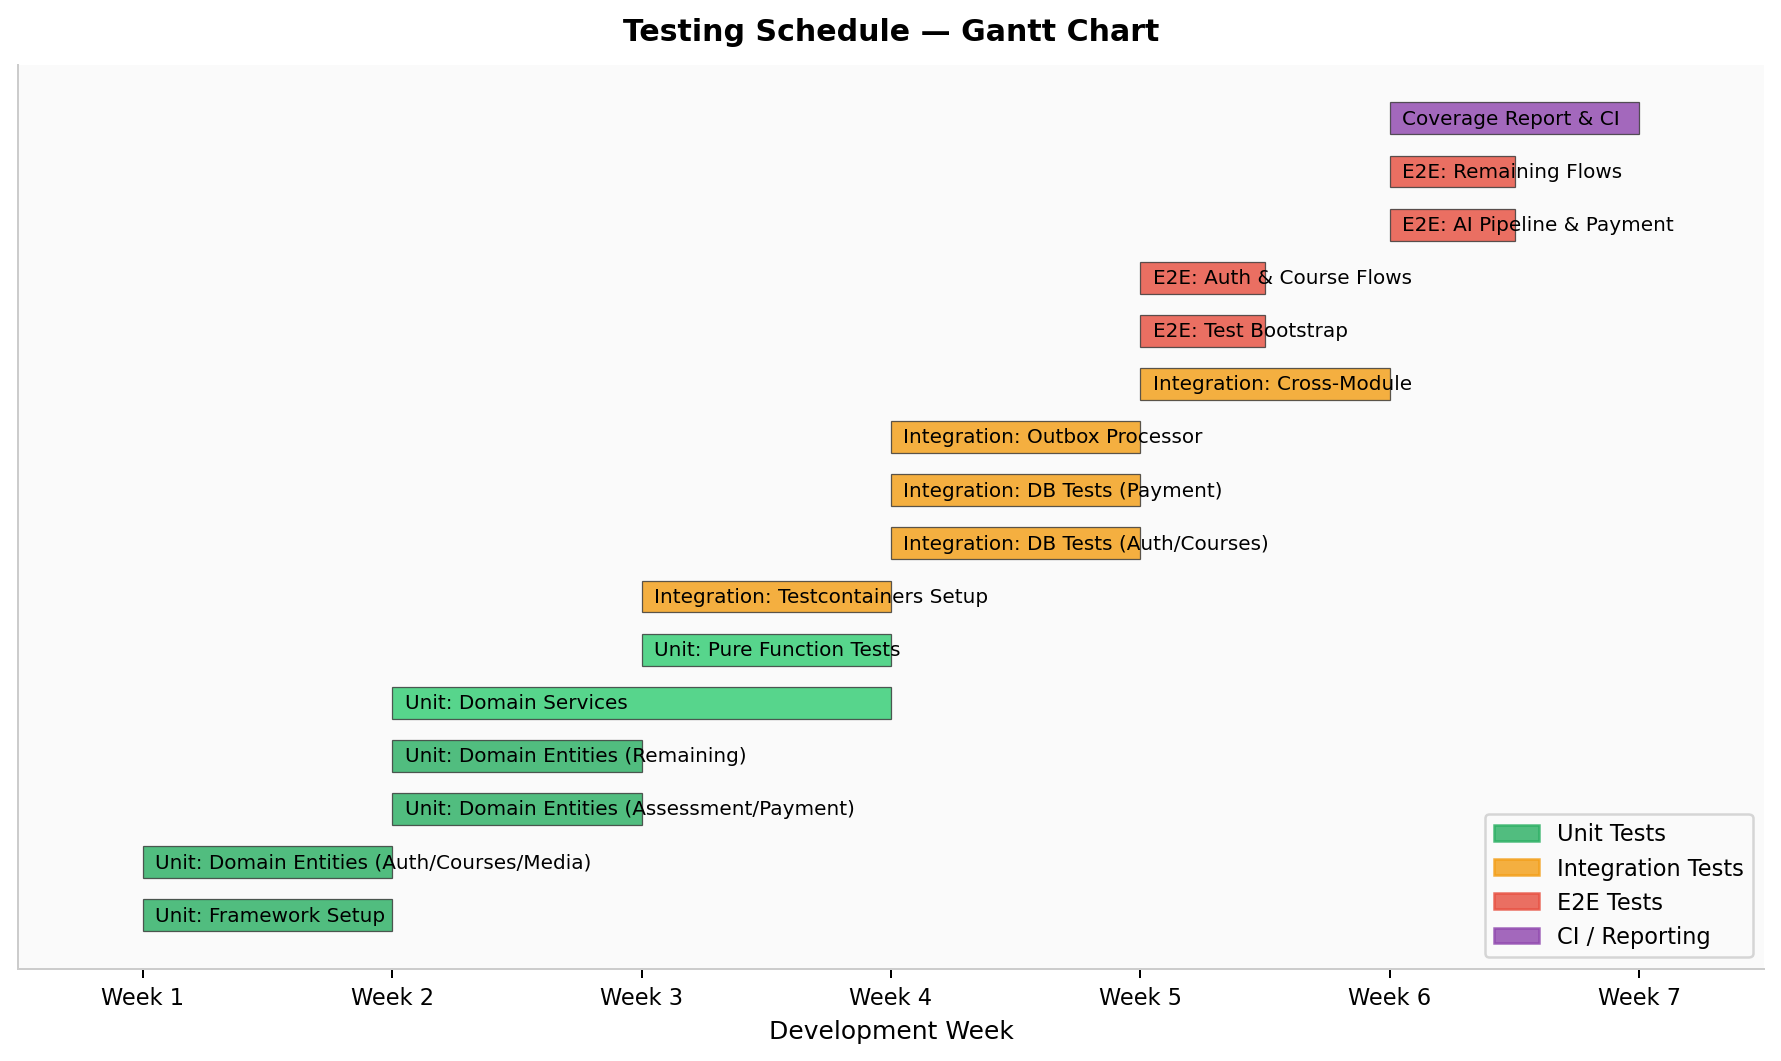
\includegraphics[width=0.75\textwidth]{images/test_schedule_gantt.png}
  \caption{Gantt chart visualisation of the testing schedule, showing the parallel execution of unit tests across bounded contexts followed by sequential integration and E2E phases.}\label{fig:test-schedule}
\end{figure}
